\documentclass[12pt,a4paper,]{article}
\usepackage[]{accanthis}
\usepackage{amssymb,amsmath}
\usepackage{ifxetex,ifluatex}
\usepackage{fixltx2e} % provides \textsubscript
\ifnum 0\ifxetex 1\fi\ifluatex 1\fi=0 % if pdftex
  \usepackage[T1]{fontenc}
  \usepackage[utf8]{inputenc}
\else % if luatex or xelatex
  \ifxetex
    \usepackage{mathspec}
  \else
    \usepackage{fontspec}
  \fi
  \defaultfontfeatures{Ligatures=TeX,Scale=MatchLowercase}
\fi
% use upquote if available, for straight quotes in verbatim environments
\IfFileExists{upquote.sty}{\usepackage{upquote}}{}
% use microtype if available
\IfFileExists{microtype.sty}{%
\usepackage[]{microtype}
\UseMicrotypeSet[protrusion]{basicmath} % disable protrusion for tt fonts
}{}
\PassOptionsToPackage{hyphens}{url} % url is loaded by hyperref
\usepackage[unicode=true]{hyperref}
\PassOptionsToPackage{usenames,dvipsnames}{color} % color is loaded by hyperref
\hypersetup{
            pdftitle={Functional diversity of ocean microbiomes.},
            pdfauthor={Dustin Michels},
            colorlinks=true,
            linkcolor=Maroon,
            citecolor=Blue,
            urlcolor=Blue,
            breaklinks=true}
\urlstyle{same}  % don't use monospace font for urls
\usepackage[top=1.5cm, bottom=2.5cm, left=1.5cm, right=1.5cm]{geometry}
\usepackage{longtable,booktabs}
% Fix footnotes in tables (requires footnote package)
\IfFileExists{footnote.sty}{\usepackage{footnote}\makesavenoteenv{long table}}{}
\usepackage{graphicx,grffile}
\makeatletter
\def\maxwidth{\ifdim\Gin@nat@width>\linewidth\linewidth\else\Gin@nat@width\fi}
\def\maxheight{\ifdim\Gin@nat@height>\textheight\textheight\else\Gin@nat@height\fi}
\makeatother
% Scale images if necessary, so that they will not overflow the page
% margins by default, and it is still possible to overwrite the defaults
% using explicit options in \includegraphics[width, height, ...]{}
\setkeys{Gin}{width=\maxwidth,height=\maxheight,keepaspectratio}
\setlength{\emergencystretch}{3em}  % prevent overfull lines
\providecommand{\tightlist}{%
  \setlength{\itemsep}{0pt}\setlength{\parskip}{0pt}}
\setcounter{secnumdepth}{0}
% Redefines (sub)paragraphs to behave more like sections
\ifx\paragraph\undefined\else
\let\oldparagraph\paragraph
\renewcommand{\paragraph}[1]{\oldparagraph{#1}\mbox{}}
\fi
\ifx\subparagraph\undefined\else
\let\oldsubparagraph\subparagraph
\renewcommand{\subparagraph}[1]{\oldsubparagraph{#1}\mbox{}}
\fi

% set default figure placement to htbp
\makeatletter
\def\fps@figure{htbp}
\makeatother

% \usepackage[vmargin=1in,hmargin=1in]{geometry}
% \usepackage{lineno}
% \linenumbers
% \usepackage{times}

\title{Functional diversity of ocean microbiomes.}
\author{Dustin Michels}
\date{Nov 2017}

\begin{document}
\maketitle

\section{Abstract}\label{abstract}

No abstract yet\ldots{}

\section{Introduction}\label{introduction}

There are important differences

When comparing communities of macroorganismal organisms, one might
compute metrics of species diversity. In microbial communities however,
species are harder to define, in part due to the frequency with which
horizontal gene transfer occurs. Some have suggested shifting focus away
from the notion of species towards distributions of genes, when
evaluating microbial communities. {[}1{]}.

Furthermore, while geographic isolation is considered a major factor in
determining the distinctiveness of macroorganismal populations,
microbiology has long entertained the hypothesis that `everything is
everywhere: but the environment selects'-- articulated by Lourens G. M.
Baas Becking in 1934 {[}1{]}. If taxonomy is

Thus, one question in microbiology is what can

Various microbiomes

``Functional redundancy''

has been observed in many environments

The idea t-- remained a widespread and well-regarded feature of
microbiological throughout the 20th century.

Various authors have found that differences in taxonomic composition
reveal less about the particular physicochemically of an ecosystem than
differences in functional composition.{[}2{]}.

In this paper, we use metagenomics first to characterize taxonomic and
functional diversity across eleven disparate Tara Ocean samples, and
evaluate evidence of functional redundancy. Secondly, we will
investigate environmental drivers of taxonomic and functional diversity,
and especially whether environmental or geographic factors play a more
important role. It is expected that functional redundancy will
observable, and that environmental factors will prove a better
differentiator of both functional and taxonomic diversity than
geographic location.

In their 2015 paper ``Structure and function of the global ocean
microbiome'', Sunagawa et al., analyzed metagenomic data from 243
\emph{Tara Oceans} samples from around the world, in part to
characterize the oceans taxonomic and functional diversity, and consider
factors that could be driving taxonomic and functional stratification.

\begin{itemize}
\tightlist
\item
  temp and diversity
\end{itemize}

"

Differences in metabolic function among organisms are thought to
underlie much of this variation as a result of selection for specific
metabolic pathways based on physicochemical conditions (``metabolic
niche effects'' or ``environmental filtering'').

However, other factors such as biotic interactions (5--7), limits to
spatial dispersal (4), and neutral demo- graphic drift (8) could also
affect community composition``{[}2{]}.

which factors drive strafaction of taxonomic and functional groups

``However, the recent claim that geographical barriers do not exist for
any micro-organism (Finlay 2002) has renewed the search for examples of
`microbial marsupials' (Fenchel 2003).'' {[}3{]}

``In general, environmental conditions strongly predicted the functional
profiles of microbial communities but weakly predicted the taxonomic
composition''{[}2{]}

``most environmental variables either correlated more strongly with
relative functional group abundances than with OTU proportions within
functional groups

" In particular, an organism's metabolic potential appears to be the
main trait selected for by environmental conditions across the global
ocean.``''

One paper that addresses these questions is ``Structure and fucntion of
global ocean microbiome'' by Sunagawa et al. {[}4{]}.

``The bulk of global biogeochemical fluxes is driven by a core set of
metabolic pathways that evolved in response to past geochemical condi-
tions (1). Through time, these pathways have spread across microbial
clades that compete within metabolic niches, resulting in an enormous
microbial diversity characterized by high functional redundancy''{[}2{]}

This project is inspired by the paper ``Structure and function of the
global ocean microbiome'' by Sunagawa et al. {[}4{]}, as well as the
paper ``An obesity-associated gut microbiome with increased capacity for
energy harvest'' by Turnbaugh et al. {[}{\textbf{???}}{]}. The first
paper seeks to characterize staxonomic differences and differences in
gene function between ocean microbiomes, using Tara Ocean samples from
around the world. They seek to identify which factors could best explain
that variation. The second paper, by Turnbaugh et al., at one point
describes the differences between the distal gut microbiomes of mice
using functional annotations of the various microbiomes, and visualizes
the result using heat maps.

My goal in this paper was to employ some of the tactics of the Turnbaugh
et al paper-- understanding the functional differences between
metagenomes using heat maps-- to the domain of the Sunagawa et al.
paper, characterizing functional differences between ocean regions.

Questions: * Which are the dominant functional and taxonomic groups? *

One thing to note: I am interested in the challenge of ensuring
reproducibility in bioinformatics projects, and have attempted to
structure this investigation for maximum reproducibility. Namely,

\begin{itemize}
\tightlist
\item
  All files are being stored (at various stages) using a public GitHub
  repository (See:
  \url{https://github.com/dustinmichels/biol338-final-project/tree/master}).
  The code associated with this draft is tagged as ``draft01'' and be
  retrieved in its entirety from GitHub.
\item
  I am attempting to carry out most stages of data collection, analysis,
  and presentation, using scripts that should be viable to re-run on
  other machines at other times to generate the same results. Even this
  report is being written in plain-text (Markdown) and converted into a
  report using a tool called Pandoc!
\item
  Finally, I am taking care to document the software I am using, and
  which version I am using, and how I am using it.
\end{itemize}

\section{Materials \& Methods}\label{materials-methods}

\subsection{Data}\label{data}

I have

I have used the eleven Tara Ocean samples that our class has used
throughout the term, but I have downloaded Gene Ontology (GO) files for
each dataset, which detail the number of reads from that dataset that
mapped to each of about 2000 different functional categories, pertaining
to molecular function, cellular components, or biological processes.

For each dataset, I normalized the `read count' into a `read proportion'
(the number of reads that mapped to a given functional category out of
all the reads.) I then selected the top 30 most abundant functional
categories, for each dataset. I ended up dropping three of these
functional categories from my analysis, which had missing data for one
or more samples. That is to say, I wound up plotting the \emph{union} of
the 30 most abundant functional groups from each sample, which is 27
functional groups.

I created three heat maps, one for all eleven samples, one grouped by
region, and one grouped by zone.

I then created three ``cluster maps.'' A cluster map is similar to a
heat map, except it clusters data hierarchically. It calculates pairwise
Euclidean distance between observations in n-dimensional space, and
groups closely related attributes together. It rearranges data
accordingly, and even draws tree structures resembling phylogenies to
indicate groupings. This method produced pretty interesting results, but
I will need to further investigate exactly how this works to ensure the
results are meaningful.

\begin{figure}
\centering
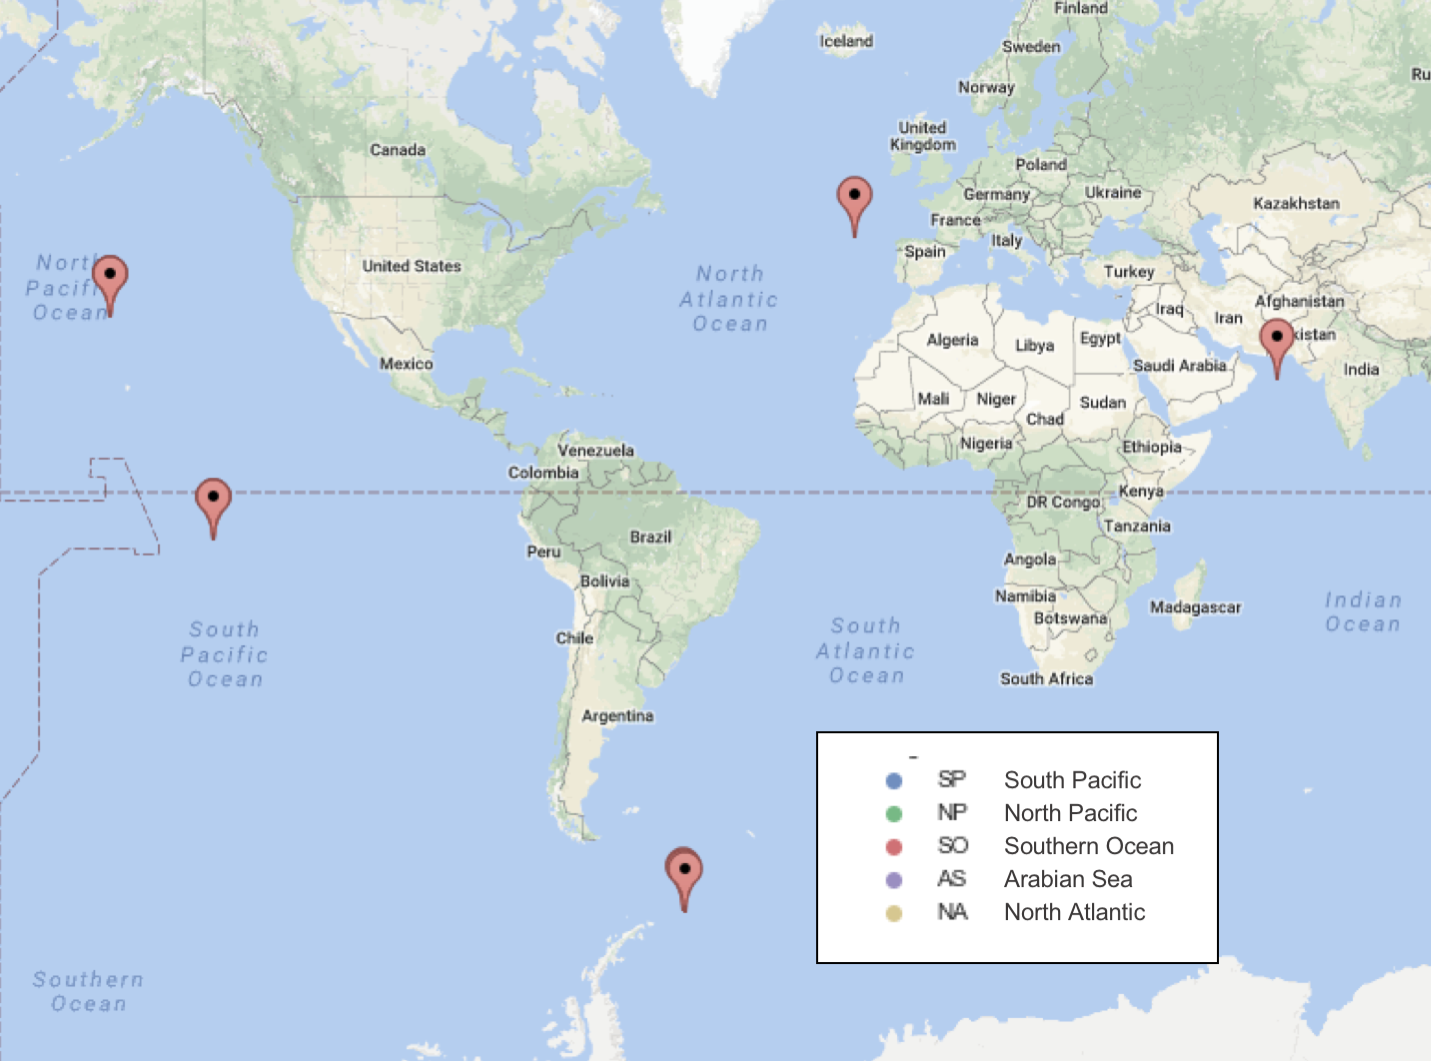
\includegraphics{imgs/map.png}
\caption{Map of sample sites.\label{fig:map}}
\end{figure}

The exact steps I took to do this analysis can be seen and reproduced
on-line at \url{http://bit.ly/2zEMitP}.

\subsection{Functional Annotations}\label{functional-annotations}

EMBL-EBI GO annotations. Gene Ontology (GO) terms derived from InterPro
matches to your sample.

\subsection{Taxonomy}\label{taxonomy}

Mothur (version 1.38.1)

Notes on exact commands are available at:
https://github.com/dustinmichels/biol338-final-project/tree/master/data/taxonomy

classified against to SILVA database

\subsection{Further Analysis and
Plotting}\label{further-analysis-and-plotting}

11 Samples. Downloaded Complete GO annotation

EBI Metagenomics

https://www.ebi.ac.uk

\section{Results}\label{results}

Here are the heat maps and cluster maps that I generated.

\begin{figure}
\centering
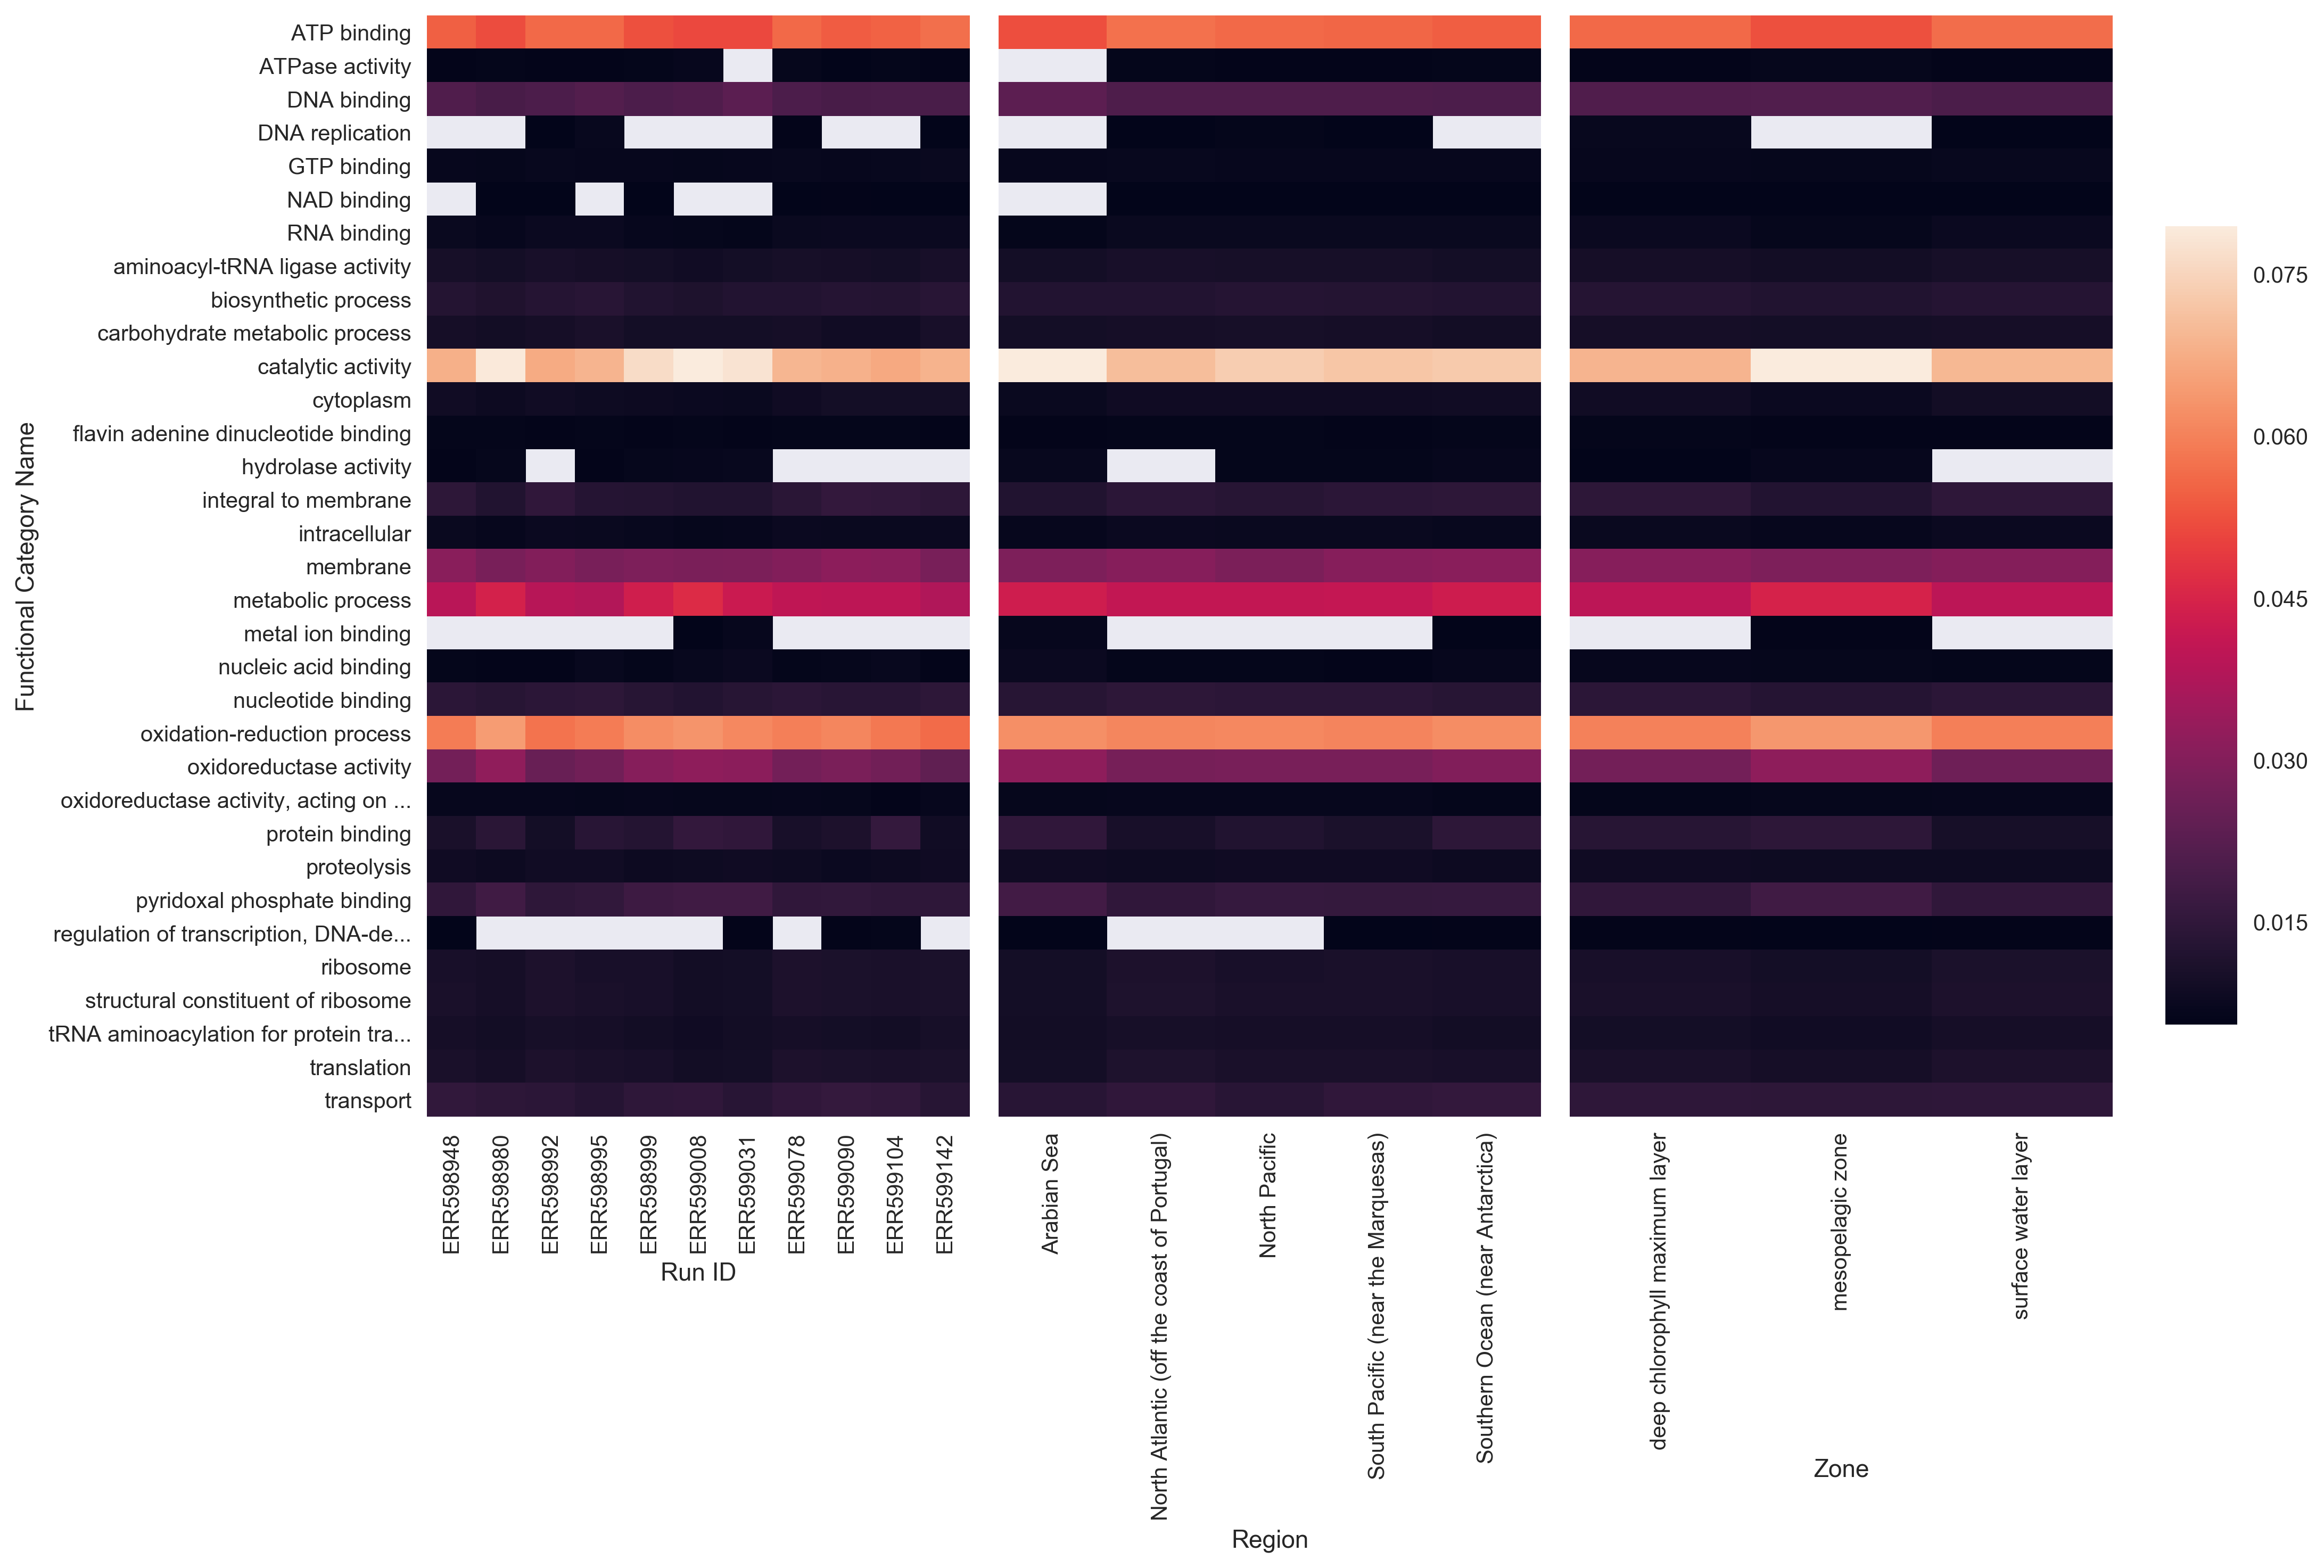
\includegraphics{imgs/heat/heat_group.png}
\caption{Heat map for all samples, and for samples grouped by region,
and for samples by grouped by zone. The top 30 most abundant functional
groups are on the vertical axis, and the proportion of reads that mapped
to that functional group is shown by the heat map
color.\label{fig:heat_group}}
\end{figure}

\begin{figure}
\centering
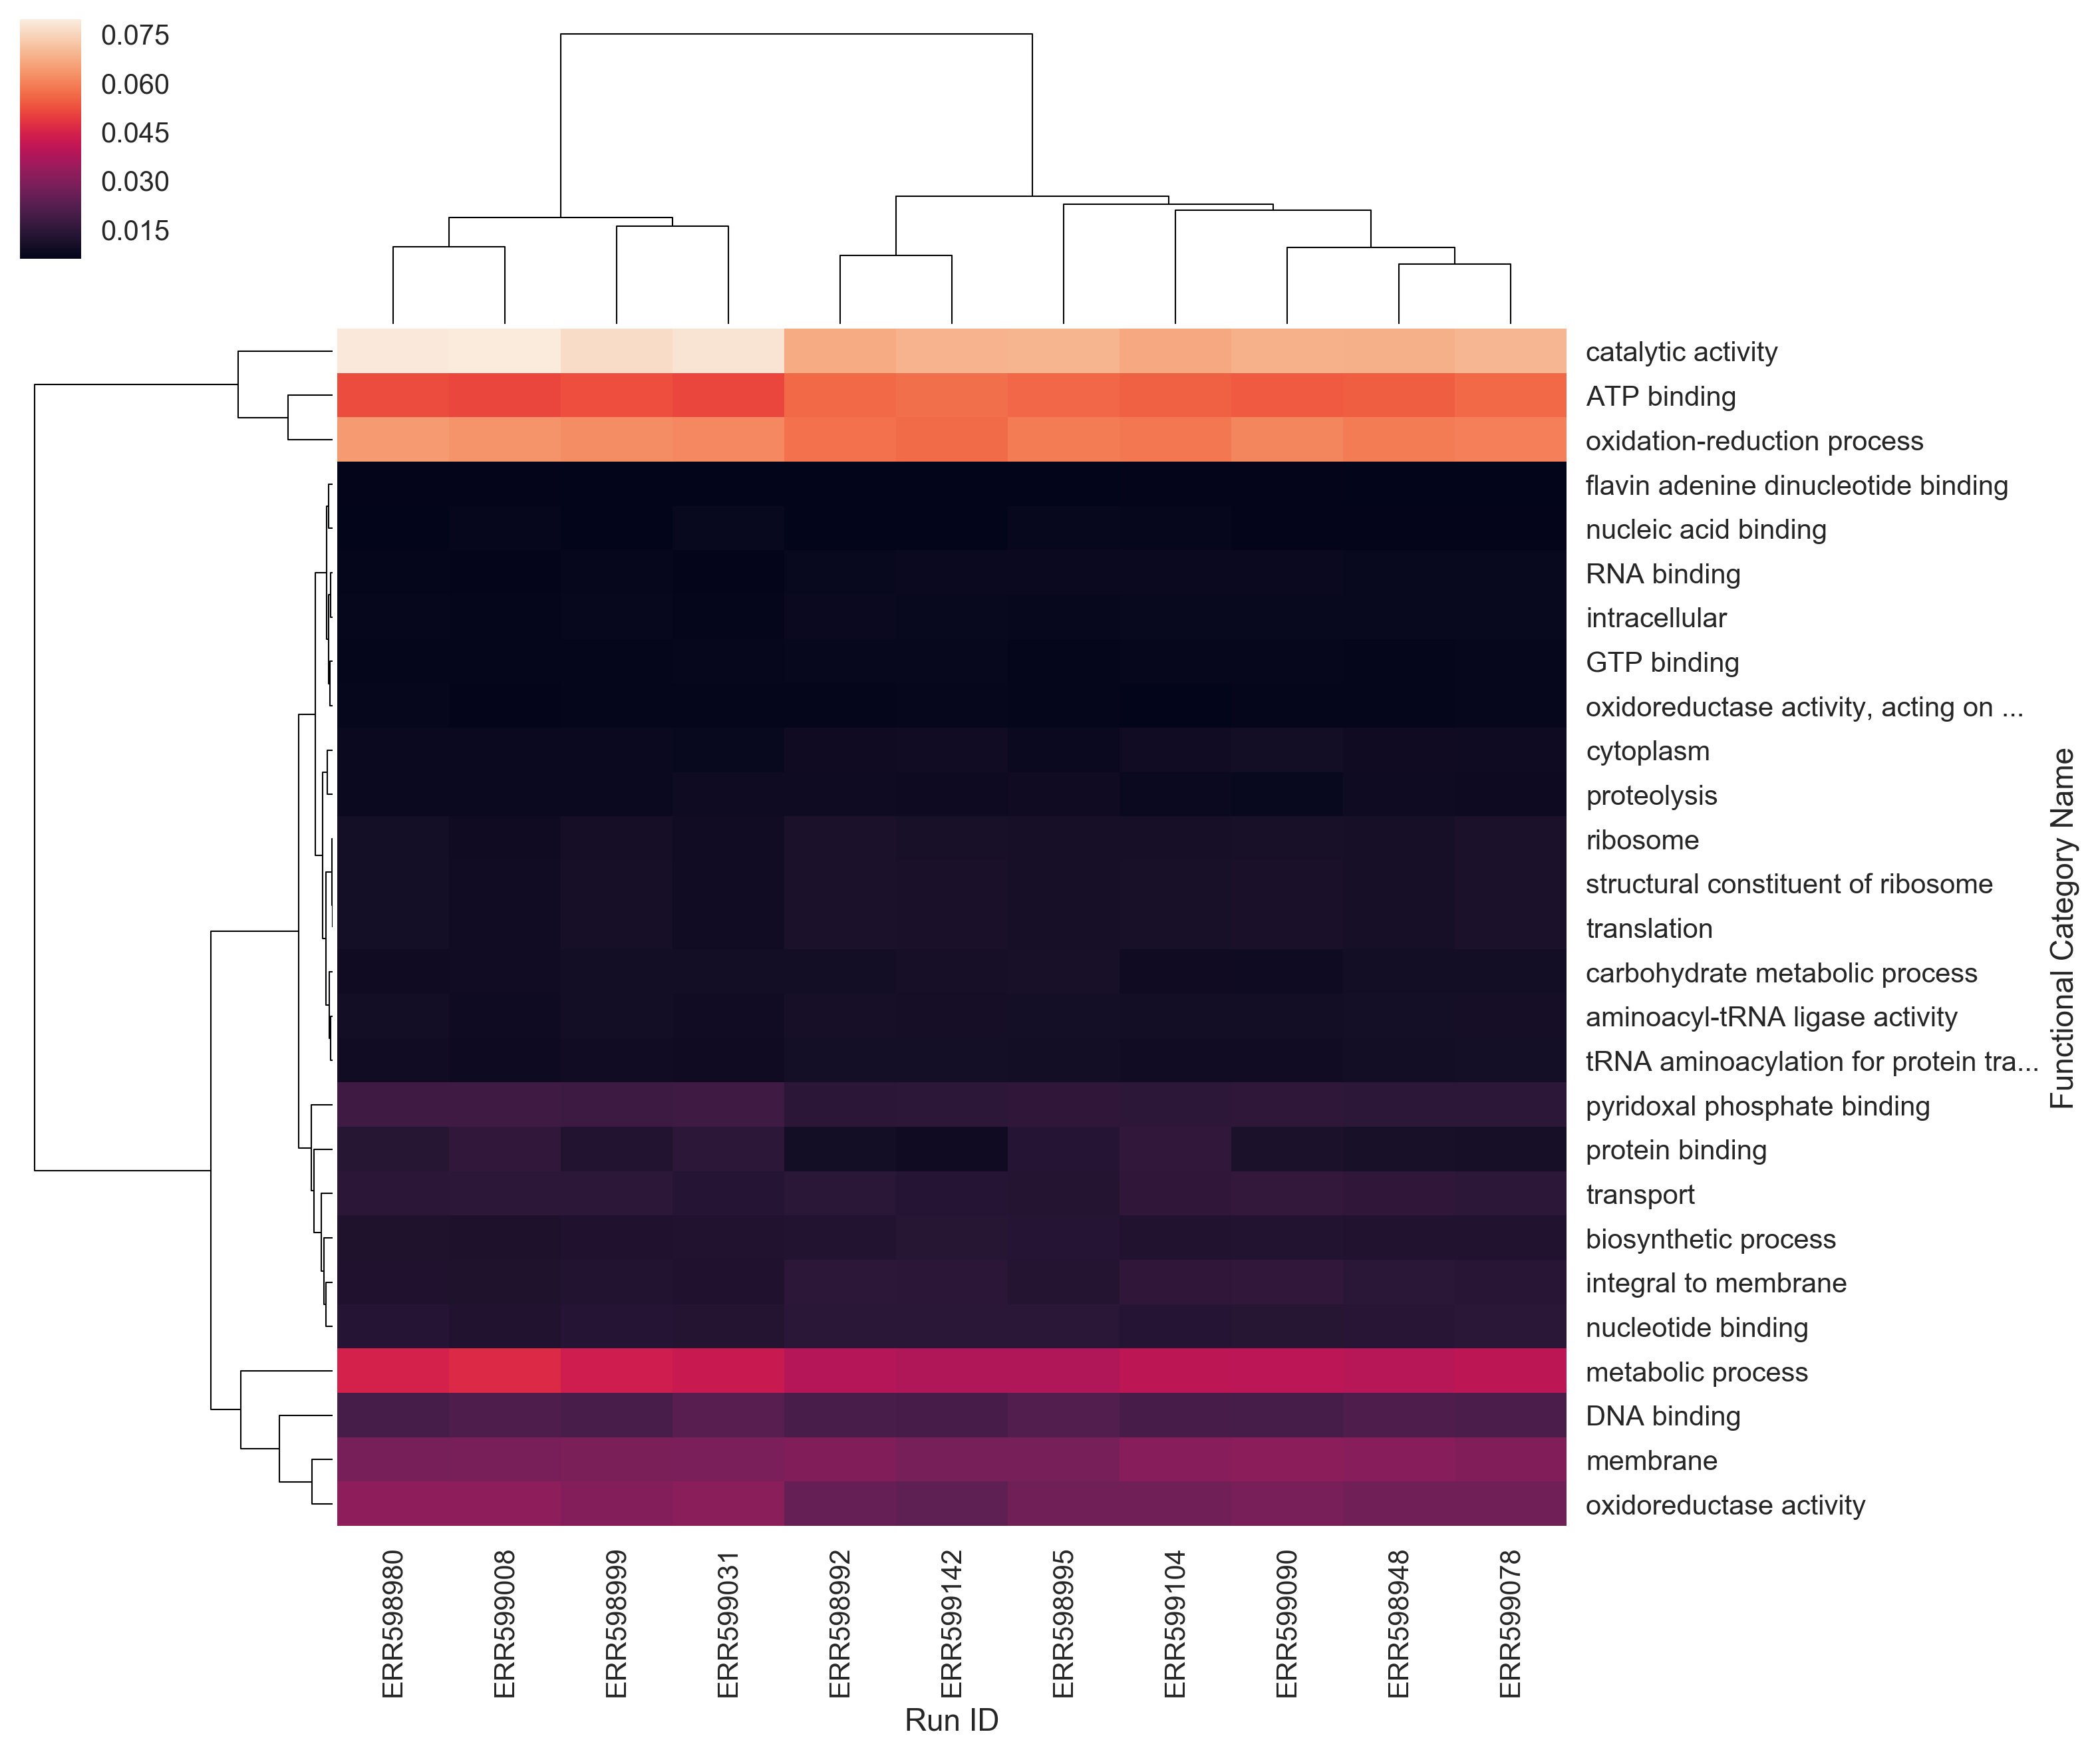
\includegraphics{imgs/cluster/cluster_all.png}
\caption{Cluster map for all samples\label{fig:cluster_all}}
\end{figure}

\begin{figure}
\centering
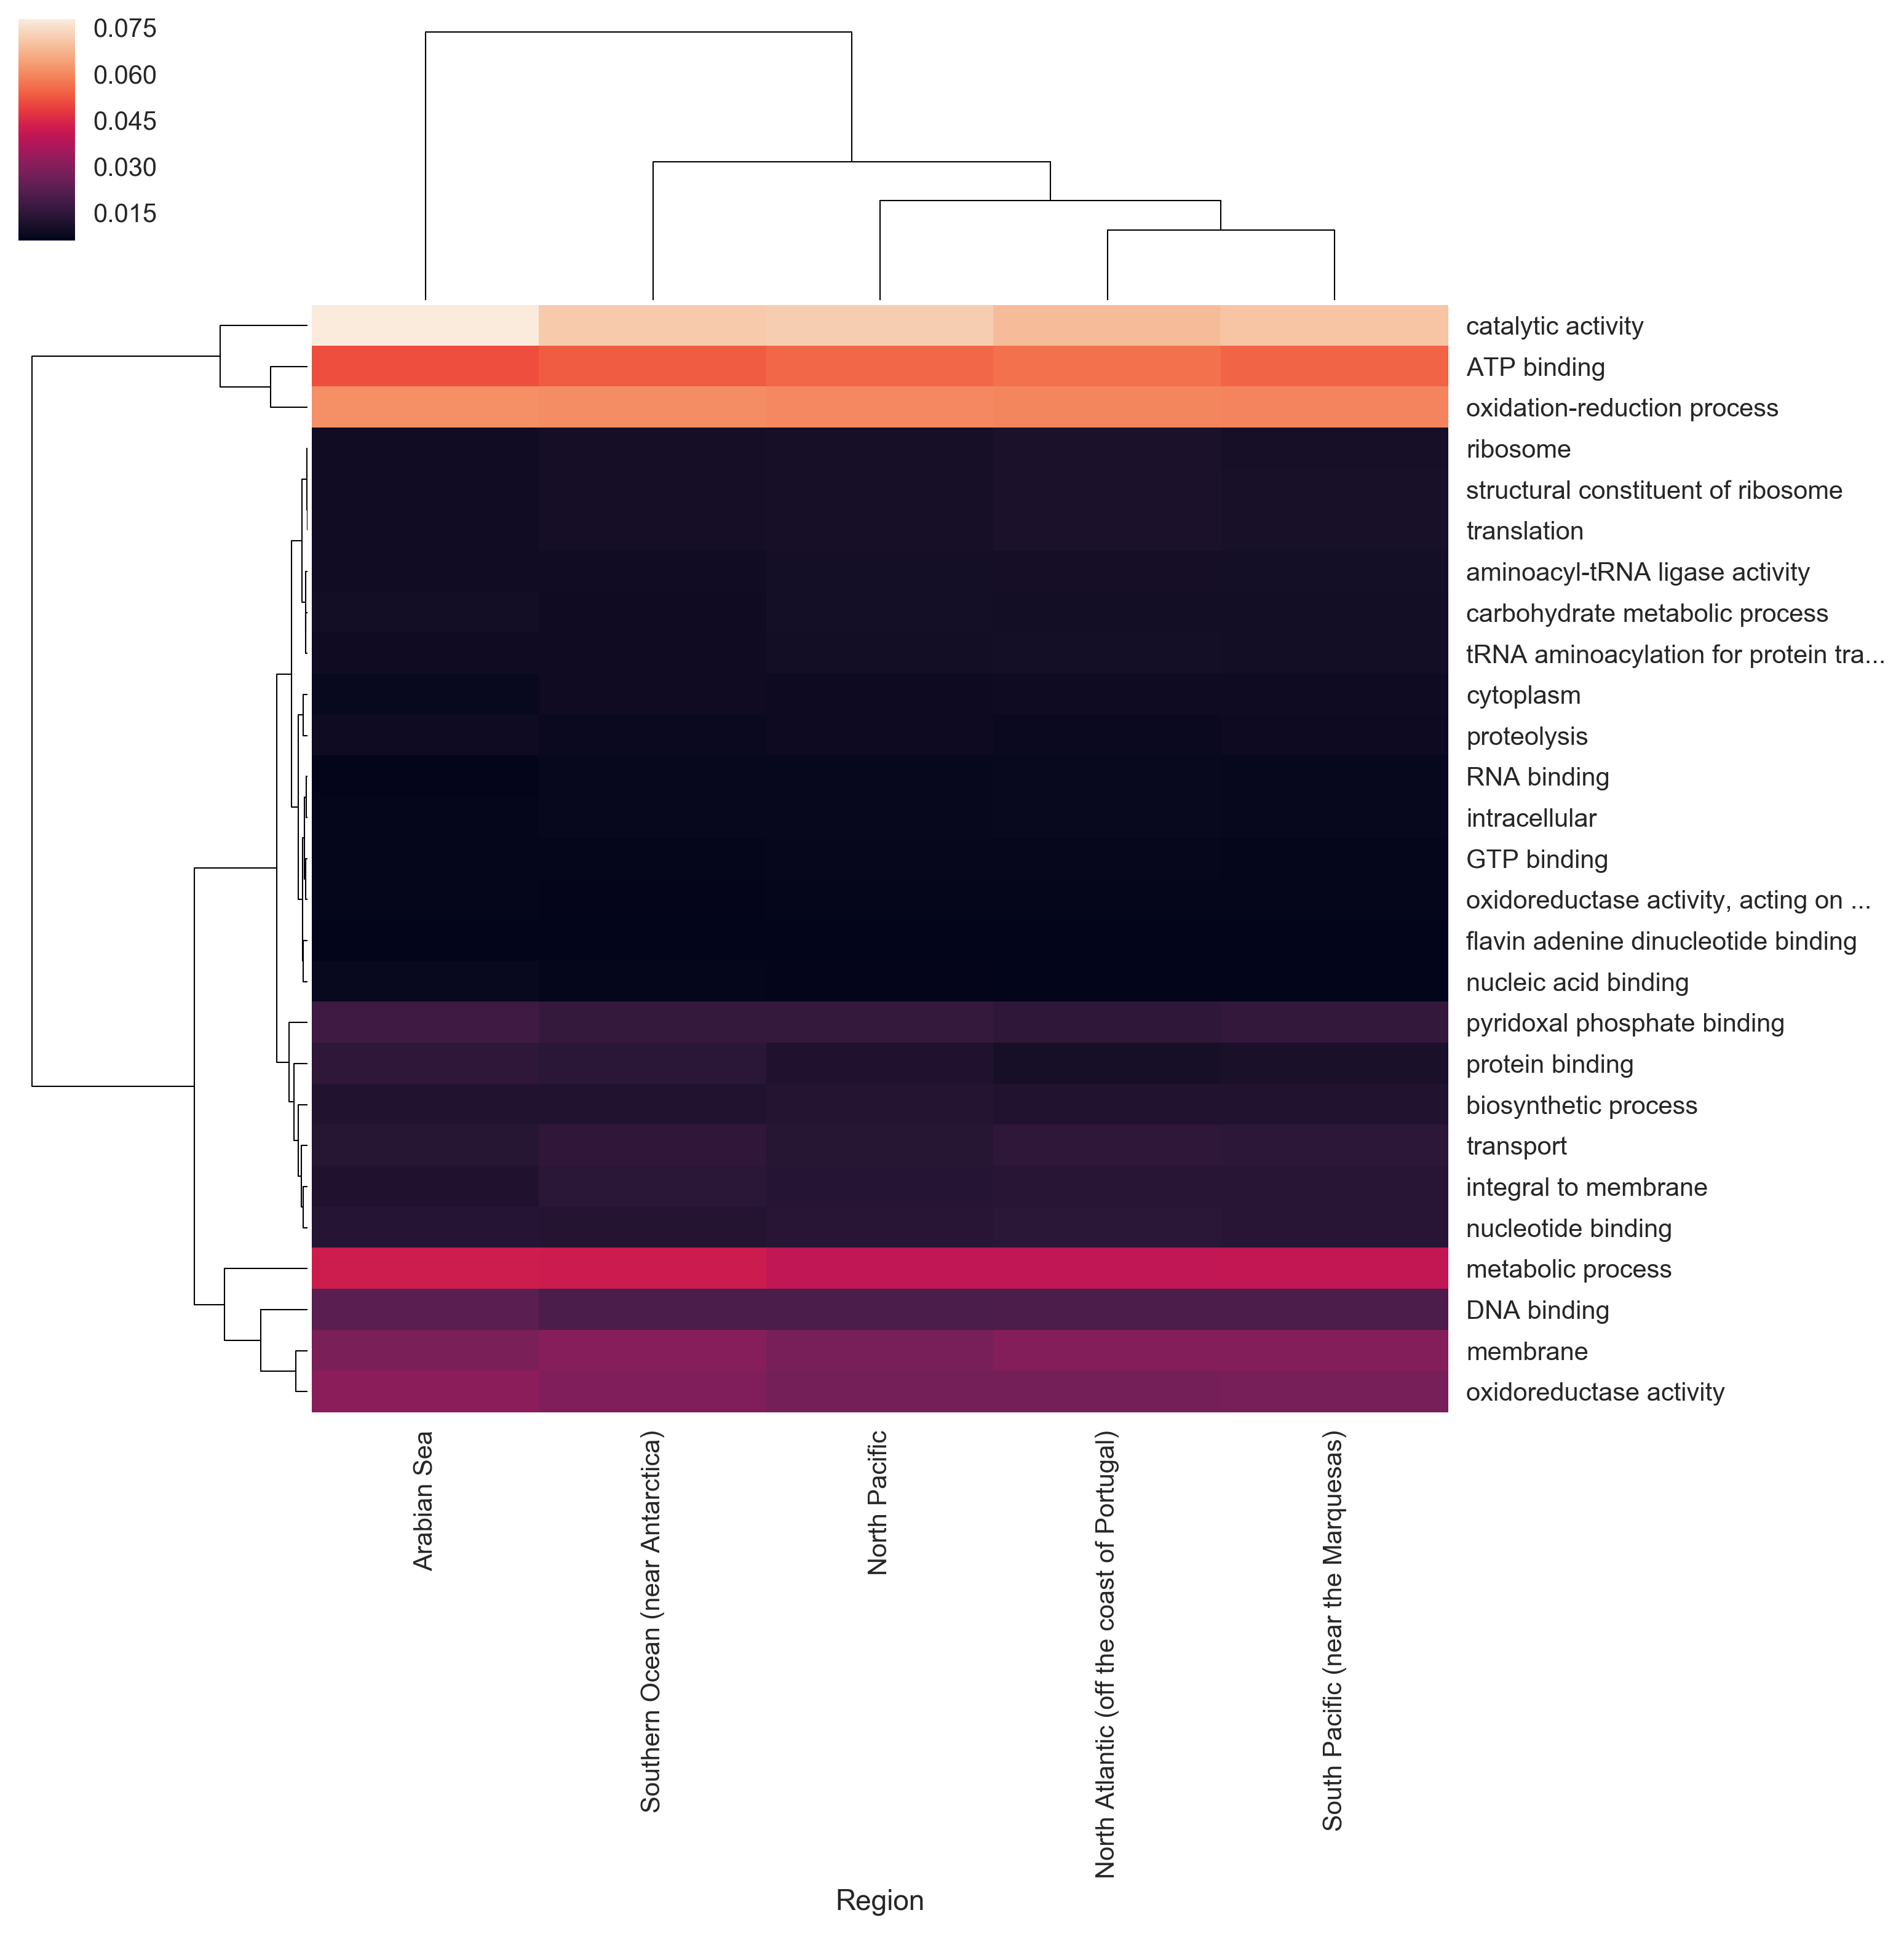
\includegraphics{imgs/cluster/cluster_region.png}
\caption{Cluster map, grouped by region\label{fig:cluster_region}}
\end{figure}

\begin{figure}
\centering
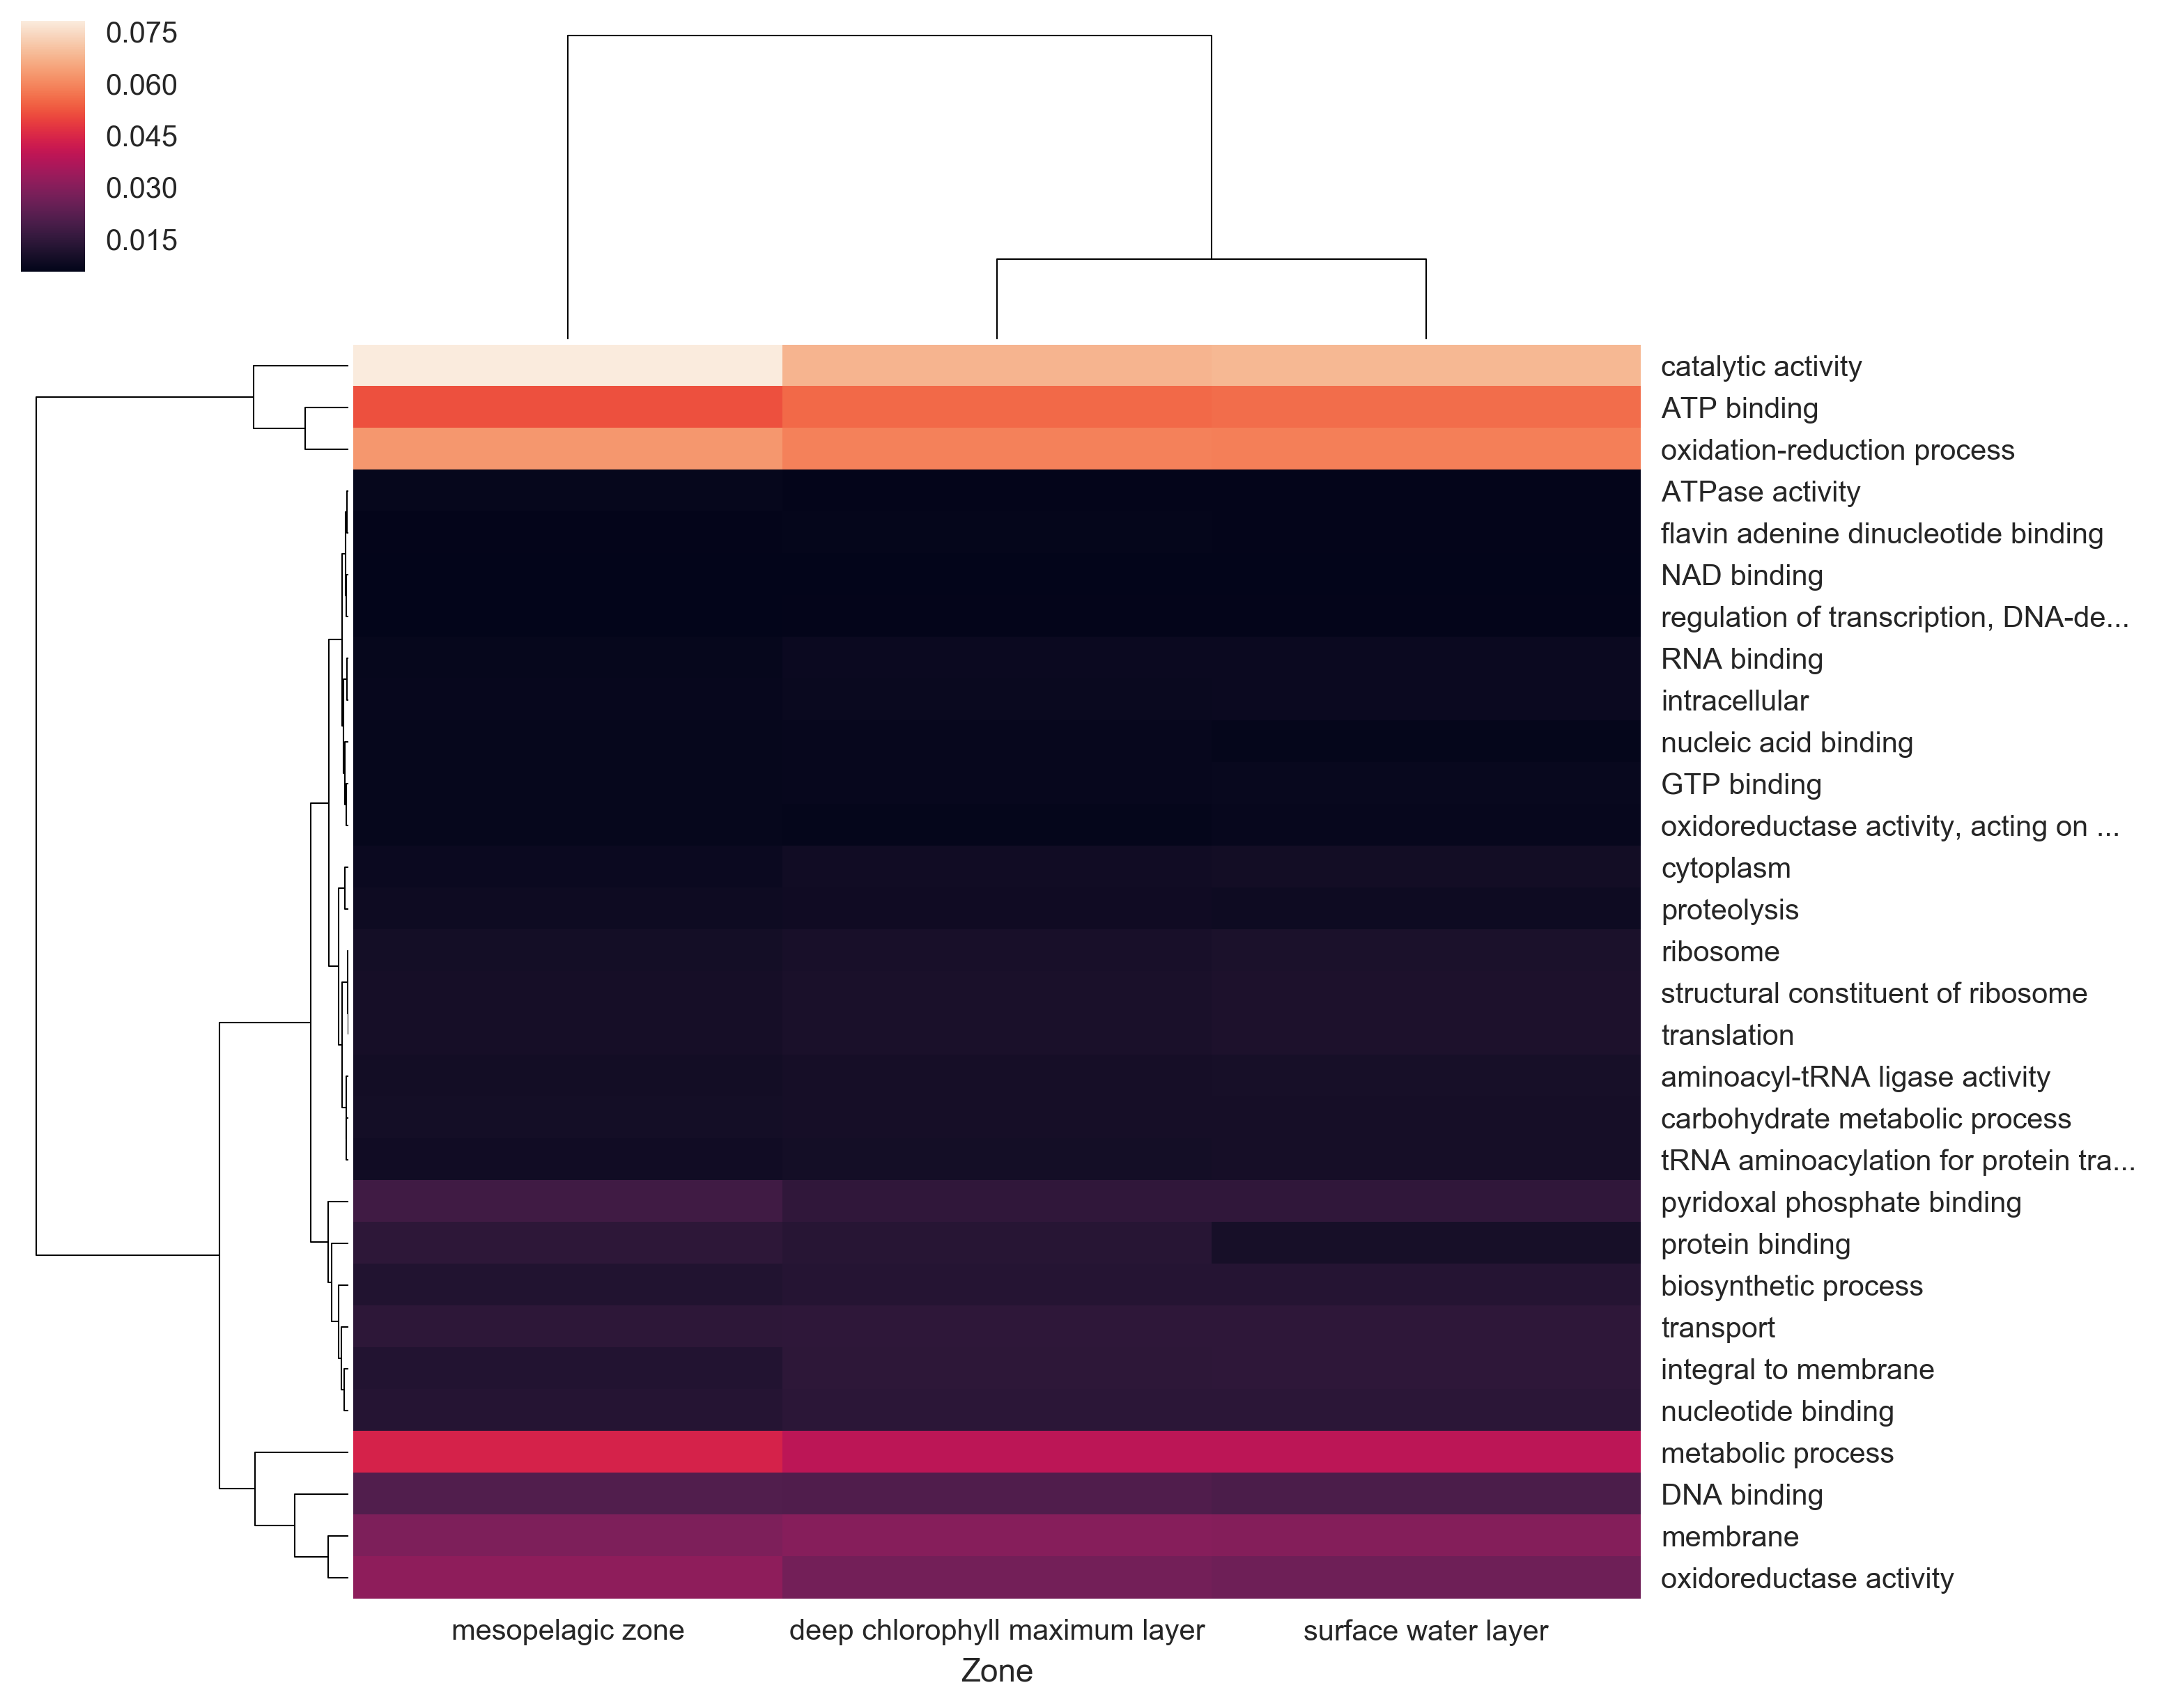
\includegraphics{imgs/cluster/cluster_zone.png}
\caption{Cluster map, grouped by zone\label{fig:cluster_zone}}
\end{figure}

\subsubsection{Heat / Cluster}\label{heat-cluster}

\begin{itemize}
\tightlist
\item
  Functional diversity smoother than taxonomic
\end{itemize}

\subsubsection{Joint}\label{joint}

\begin{itemize}
\tightlist
\item
  Functional diversity correlated with
\end{itemize}

The fact that depth captures diversity better than other metadata may
suggest that there is an aspect to ``depth'' not captured by the other
variables.

OCEAN PAPER:

They suggest that temperature and light have stronger effects on
functional trait composition than nutrients or salinity.

Taxonomic compositions do not show a clear separation by regional origin

Global ocean paper suggests ``increase in taxonomic and functional''
richness with depth.

The idea that the

\section{Discussion}\label{discussion}

The cluster maps seem to suggest that deep chlorophyll maximum layer and
the surface water later are more closely related to each other, in terms
of prevalence of functional gene categories, prevalence than either is
to the mesopelagic zone

Similarly, the cluster maps would suggest that the North Atlantic and
South Atlantic are the most functionally similar, followed by the North
Pacific, followed by the Souther Ocean, and finally the Arabian Sea.

More analysis underway!

They stated members of Proteobacteria, including Alphaproteobacteria and
Gammaproteobacteria, as well as Cyanobacteria, Deferribacteres, and
Thaumarchaeota.

For me, temperature shadowed by depth.

Functional redundancy. (including Cyanobacteria, De)

``This has implications for the interpretation of differences in
community structure across envi- ronments and time. Differences in
taxonomic composition that do not affect functional com- position may
have little relevance to ecosystem biochemistry; conversely,
physicochemically sim- ilar environments could host taxonomically dis-
tinct communities (26). Functional (rather than purely taxonomic)
descriptions of microbial com- munities should therefore constitute the
baseline for microbial biogeography, particularly across transects where
geochemical gradients shape microbial niche distribution''{[}2{]}

\subsection{Further Research}\label{further-research}

\begin{itemize}
\tightlist
\item
  Look at relatedness of species? (more related across depths or
  regions?)
\end{itemize}

\section{References}\label{references}

\hypertarget{refs}{}
\hypertarget{ref-omalley_everything_2008}{}
1. O'Malley MA. ``Everything is everywhere: But the environment
selects'': Ubiquitous distribution and ecological determinism in
microbial biogeography. Studies in History and Philosophy of Science
Part C: Studies in History and Philosophy of Biological and Biomedical
Sciences. 2008;39: 314--325.
doi:\href{https://doi.org/10.1016/j.shpsc.2008.06.005}{10.1016/j.shpsc.2008.06.005}

\hypertarget{ref-louca_decoupling_2016}{}
2. Louca S, Parfrey LW, Doebeli M. Decoupling function and taxonomy in
the global ocean microbiome. Science. 2016;353: 1272--1277.
doi:\href{https://doi.org/10.1126/science.aaf4507}{10.1126/science.aaf4507}

\hypertarget{ref-whitaker_allopatric_2006}{}
3. Whitaker RJ. Allopatric origins of microbial species. Philosophical
Transactions of the Royal Society B: Biological Sciences. 2006;361:
1975--1984.
doi:\href{https://doi.org/10.1098/rstb.2006.1927}{10.1098/rstb.2006.1927}

\hypertarget{ref-sunagawa_structure_2015}{}
4. Sunagawa S, Coelho LP, Chaffron S, Kultima JR, Labadie K, Salazar G,
et al. Structure and function of the global ocean microbiome. Science.
2015;348: 1261359.
doi:\href{https://doi.org/10.1126/science.1261359}{10.1126/science.1261359}

\section{Appendix}\label{appendix}

\tiny

\begin{longtable}[]{@{}lll@{}}
\caption{For each sample, a `Reads encoding 5S rRNA' file and a
`Complete GO annotation' file was downloaded from the given link.
\label{tbl:docs}}\tabularnewline
\toprule
\begin{minipage}[b]{0.08\columnwidth}\raggedright\strut
Run ID\strut
\end{minipage} & \begin{minipage}[b]{0.15\columnwidth}\raggedright\strut
Description\strut
\end{minipage} & \begin{minipage}[b]{0.69\columnwidth}\raggedright\strut
Link\strut
\end{minipage}\tabularnewline
\midrule
\endfirsthead
\toprule
\begin{minipage}[b]{0.08\columnwidth}\raggedright\strut
Run ID\strut
\end{minipage} & \begin{minipage}[b]{0.15\columnwidth}\raggedright\strut
Description\strut
\end{minipage} & \begin{minipage}[b]{0.69\columnwidth}\raggedright\strut
Link\strut
\end{minipage}\tabularnewline
\midrule
\endhead
\begin{minipage}[t]{0.08\columnwidth}\raggedright\strut
ERR599104\strut
\end{minipage} & \begin{minipage}[t]{0.15\columnwidth}\raggedright\strut
Southern Ocean (DCM)\strut
\end{minipage} & \begin{minipage}[t]{0.69\columnwidth}\raggedright\strut
https://www.ebi.ac.uk/metagenomics/projects/ERP001736/samples/ERS491095/runs/ERR599104/results/versions/2.0\strut
\end{minipage}\tabularnewline
\begin{minipage}[t]{0.08\columnwidth}\raggedright\strut
ERR599090\strut
\end{minipage} & \begin{minipage}[t]{0.15\columnwidth}\raggedright\strut
Southern Ocean (SURF)\strut
\end{minipage} & \begin{minipage}[t]{0.69\columnwidth}\raggedright\strut
https://www.ebi.ac.uk/metagenomics/projects/ERP001736/samples/ERS491044/runs/ERR599090/results/versions/2.0\strut
\end{minipage}\tabularnewline
\begin{minipage}[t]{0.08\columnwidth}\raggedright\strut
ERR599008\strut
\end{minipage} & \begin{minipage}[t]{0.15\columnwidth}\raggedright\strut
Southern Ocean (MESO)\strut
\end{minipage} & \begin{minipage}[t]{0.69\columnwidth}\raggedright\strut
https://www.ebi.ac.uk/metagenomics/projects/ERP001736/samples/ERS491110/runs/ERR599008/results/versions/2.0\strut
\end{minipage}\tabularnewline
\begin{minipage}[t]{0.08\columnwidth}\raggedright\strut
ERR598948\strut
\end{minipage} & \begin{minipage}[t]{0.15\columnwidth}\raggedright\strut
South Pacific (DCM)\strut
\end{minipage} & \begin{minipage}[t]{0.69\columnwidth}\raggedright\strut
https://www.ebi.ac.uk/metagenomics/projects/ERP001736/samples/ERS492699/runs/ERR598948/results/versions/2.0\strut
\end{minipage}\tabularnewline
\begin{minipage}[t]{0.08\columnwidth}\raggedright\strut
ERR598992\strut
\end{minipage} & \begin{minipage}[t]{0.15\columnwidth}\raggedright\strut
South Pacific (SURF)\strut
\end{minipage} & \begin{minipage}[t]{0.69\columnwidth}\raggedright\strut
https://www.ebi.ac.uk/metagenomics/projects/ERP001736/samples/ERS492642/runs/ERR598992/results/versions/2.0\strut
\end{minipage}\tabularnewline
\begin{minipage}[t]{0.08\columnwidth}\raggedright\strut
ERR598999\strut
\end{minipage} & \begin{minipage}[t]{0.15\columnwidth}\raggedright\strut
South Pacific (MESO)\strut
\end{minipage} & \begin{minipage}[t]{0.69\columnwidth}\raggedright\strut
https://www.ebi.ac.uk/metagenomics/projects/ERP001736/samples/ERS492680/runs/ERR598999/results/versions/2.0\strut
\end{minipage}\tabularnewline
\begin{minipage}[t]{0.08\columnwidth}\raggedright\strut
ERR598995\strut
\end{minipage} & \begin{minipage}[t]{0.15\columnwidth}\raggedright\strut
North Pacific (DCM)\strut
\end{minipage} & \begin{minipage}[t]{0.69\columnwidth}\raggedright\strut
https://www.ebi.ac.uk/metagenomics/projects/ERP001736/samples/ERS493340/runs/ERR598995/results/versions/2.0\strut
\end{minipage}\tabularnewline
\begin{minipage}[t]{0.08\columnwidth}\raggedright\strut
ERR598980\strut
\end{minipage} & \begin{minipage}[t]{0.15\columnwidth}\raggedright\strut
North Pacific (MESO)\strut
\end{minipage} & \begin{minipage}[t]{0.69\columnwidth}\raggedright\strut
https://www.ebi.ac.uk/metagenomics/projects/ERP001736/samples/ERS493372/runs/ERR598980/results/versions/2.0\strut
\end{minipage}\tabularnewline
\begin{minipage}[t]{0.08\columnwidth}\raggedright\strut
ERR599142\strut
\end{minipage} & \begin{minipage}[t]{0.15\columnwidth}\raggedright\strut
North Pacific (SURF)\strut
\end{minipage} & \begin{minipage}[t]{0.69\columnwidth}\raggedright\strut
https://www.ebi.ac.uk/metagenomics/projects/ERP001736/samples/ERS493300/runs/ERR599142/results/versions/2.0\strut
\end{minipage}\tabularnewline
\begin{minipage}[t]{0.08\columnwidth}\raggedright\strut
ERR599078\strut
\end{minipage} & \begin{minipage}[t]{0.15\columnwidth}\raggedright\strut
North Atlantic (SURF)\strut
\end{minipage} & \begin{minipage}[t]{0.69\columnwidth}\raggedright\strut
https://www.ebi.ac.uk/metagenomics/projects/ERP001736/samples/ERS494579/runs/ERR599078/results/versions/2.0\strut
\end{minipage}\tabularnewline
\begin{minipage}[t]{0.08\columnwidth}\raggedright\strut
ERR599031\strut
\end{minipage} & \begin{minipage}[t]{0.15\columnwidth}\raggedright\strut
Arabian Sea (MESO)\strut
\end{minipage} & \begin{minipage}[t]{0.69\columnwidth}\raggedright\strut
https://www.ebi.ac.uk/metagenomics/projects/ERP001736/samples/ERS488769/runs/ERR599031/results/versions/2.0\strut
\end{minipage}\tabularnewline
\bottomrule
\end{longtable}

\end{document}
